% Chapter 1: Introduction (full)

\chapter{Introduction}
\label{ch:intro}

The project aims to improve the efficiency and safety of disaster response operations by minimizing human risk and cognitive load through an autonomous Unmanned Ground Vehicle (UGV). The UGV performs reconnaissance tasks such as mapping, hazard detection, and visual data collection, while supporting centralized and decentralized communication and AI-based perception for automated situational assessment.

The core objective is to implement LiDAR-based Simultaneous Localization and Mapping (SLAM), enabling the UGV to localize itself accurately and generate precise indoor maps. The collected data is transmitted via a multi-tier communication setup integrating Wi-Fi, mesh, and long-range radio links. To support extended missions, the UGV autonomously deploys compact mesh nodes that establish a resilient decentralized network in unstable environments.

To further reduce operator workload, the system incorporates an AI pipeline that analyzes data to identify survivors, hazards, and navigable paths, generating human-readable reports and alerts. The UGV is evaluated in controlled testing using defined Key Performance Indicators (KPIs) including localization drift, map accuracy, packet delivery ratio, network latency, detection accuracy, and reduction in operator workload.

\section{Background and Relevance}
\label{sec:background}

Disaster response robotics presents complex challenges in computation, communication, algorithms, and energy management within Computer Engineering. While mechanical robustness is essential for traversal, mission success primarily depends on effective system integration.

The first major challenge lies in real-time embedded systems and sensor fusion. Autonomous navigation requires sensor data fusion through Simultaneous Localization and Mapping (SLAM), demanding efficient algorithms capable of running on embedded hardware. Real-time acquisition, processing, and synchronization of multi-sensor data are critical to achieving accurate localization.

The second key challenge is robust communication and networking. The UGV must maintain near real-time connectivity with the operator despite indoor signal attenuation. This requires a multi-tier network combining high-bandwidth links (Wi-Fi or LTE) with a resilient decentralized mesh system. The robot deploys its own mesh nodes using an adaptive algorithm that positions them based on signal quality indicators such as RSSI and SNR.

The third challenge involves intelligent perception and Human--Robot Interaction (HRI). The system must efficiently process large data streams using AI models for visual inference and natural language summarization while minimizing latency. This processed information is presented to operators in a concise, interpretable form to enhance situational awareness and decision-making.

% --- FIGURE: Literature review taxonomy ---
\begin{figure}[htbp]
\centering
\includegraphics[width=0.75\textwidth]{figures/literature_taxonomy.jpg}
\caption{Literature review taxonomy for disaster site exploration systems.}
\label{fig:literature_taxonomy}
\end{figure}

Recent studies in this field can be categorized into three key areas: Navigation and Mapping, Resilient Communication Protocols, and Artificial Intelligence (AI) Applications.

Navigation and Mapping rely on Simultaneous Localisation and Mapping (SLAM), enabling robots to incrementally build and localize within environmental maps using LiDAR or visual data. LiDAR-based odometry performs well in low-visibility conditions but suffers from drift in sparse environments. Modern approaches mitigate this through sensor fusion using IMUs, encoders, GPS, or cameras, achieving higher precision at the cost of greater computational demand.

Communication systems critically affect the reliability of disaster response operations. Current solutions involve satellites, 5G, Software-Defined Radios (SDR), and mesh networking. Recent developments focus on hybrid, multi-tier networks that prioritize data by bandwidth and importance, transmitting it through the most suitable channel. While SDR and LoRa offer wide coverage, their limited throughput restricts high-data applications.

AI and Human--Robot Interaction (HRI) transform raw sensory data into actionable intelligence. Techniques such as object detection, map overlays, and video summarization use advanced AI/ML models, while Large Language Models (LLMs) generate mission reports and summaries. However, these methods often require GPU acceleration, making them challenging to deploy on power-constrained embedded platforms.

\section{Objectives and Deliverables}
\label{sec:objectives}

To achieve the aims outlined previously and contribute to solving the core challenges faced by UGVs, a set of objectives and measurable deliverables has been defined. These ensure the problem statement is translated into actionable tasks and outcomes that validate the project's success. The following list summarizes the core objectives and deliverables.

\begin{enumerate}
\item Implement LiDAR-based SLAM to provide localization, mapping and navigation in indoor environments.
\item Formulate a mesh-based and hybrid communication scheme and low bandwidth linking to ensure good transmission of data.
\item Integrate AI vision approaches to make sense of camera streams as well as identify items of interest and artificial intelligent summarization to create mission reports.
\item Test and integrate the UGV system to measure the key performance indicators.
\end{enumerate}

Implementing these objectives yields the following deliverables:

\begin{enumerate}
\item Autonomous UGV prototype with LiDAR-based SLAM and hybrid communication stack
\item Mesh nodes along with their deployment mechanism integrated in the UGV
\item Software stack optimized for execution on embedded hardware (Raspberry Pi~4)
\item Operator interface with maps, perception results, network status and telemetry
\end{enumerate}

% --- FIGURE: Multi-tier system architecture ---
\begin{figure}[htbp]
\centering
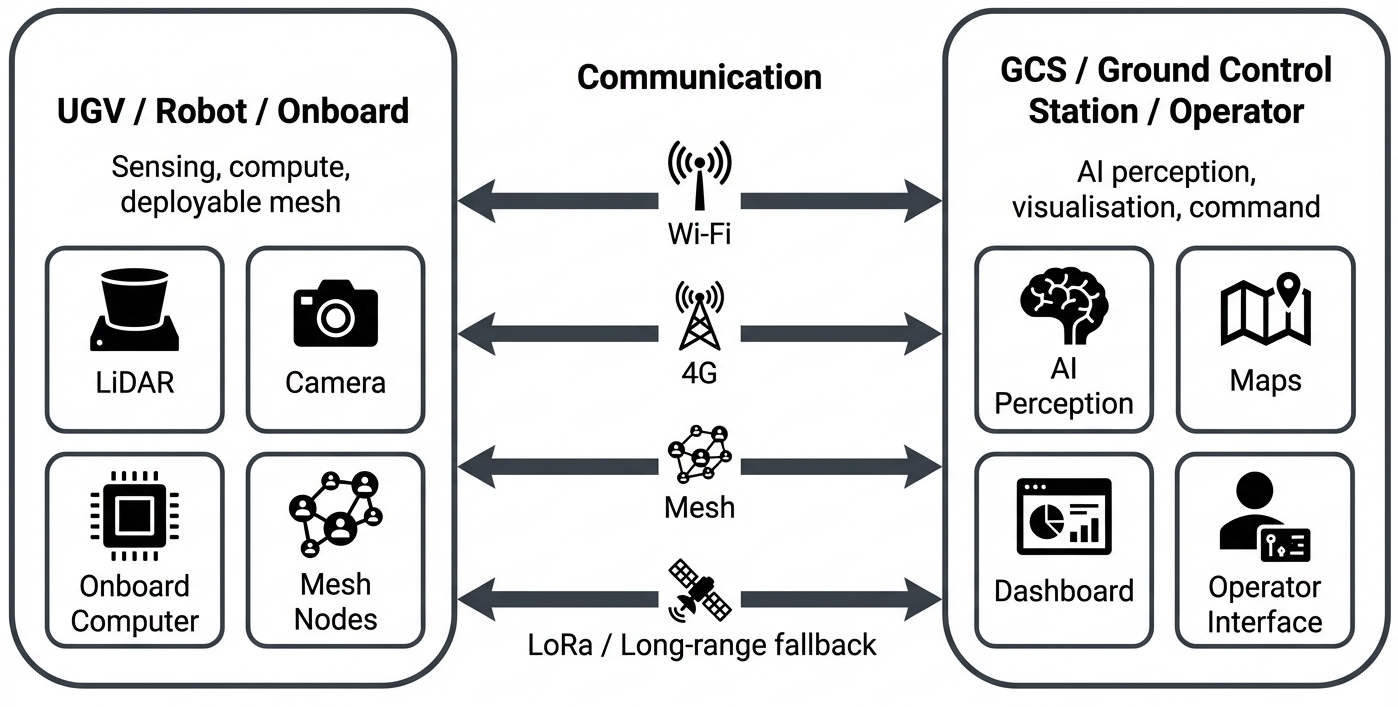
\includegraphics[width=0.8\textwidth]{figures/multitier_architecture.png}
\caption{Multi-tier system architecture for autonomous exploration with onboard sensing, mesh networking, and operator-side AI processing.}
\label{fig:multitier_arch}
\end{figure}

\section{Project Scope and Limitations}
\label{sec:scope}

The project focuses on indoor environments where GPS is unreliable, and LiDAR performs effectively without sunlight interference. A YDLidar X3 (10\,Hz) sensor supports 2D SLAM via Google Cartographer, generating 0.05\,m occupancy maps. The UGV autonomously explores with frontier-based algorithms while the Nav2 stack handles path planning and obstacle avoidance. The as-built system (Chapter~\ref{ch:impl}) covers an indoor test area of approximately 40$\times$30\,m, powered by a 24\,V pack (dual 3s3p 18650) with runtime of almost two hours at 0.2\,m/s.

A multi-tier communication framework combines ESP-WiFi-MESH as the core network with Wi-Fi, 4G, and LoRa (SX1278) as fallbacks. The UGV deploys compact mesh nodes (ESP32 DevKit, 2500\,mAh LiPo each) during exploration; nodes are added to the routing table upon deployment. AI-driven features include visual hazard detection (e.g.\ smoke, fire, extinguisher, human) and LLM-based summarisation for generating mission reports. Operators access a web dashboard offering live telemetry, map visualisation, video (720p, 15\,fps), detection overlays, and manual control. The software stack runs on ROS~2 Humble (Raspberry Pi~4 8\,GB) and ESP32 DevKit, demonstrating GPU-free autonomous operation.

The UGV handles flat surfaces with minor obstacles and supports payloads but cannot climb stairs or steep inclines. Its cameras (USB webcam and ESP32-CAM at 720p, 15\,fps) provide visual data only, lacking thermal or chemical sensing. Without wheel encoders, Cartographer's scan-matching combined with an MPU6050 IMU handles localisation, with reduced accuracy in feature-sparse spaces. The 2D SLAM system cannot detect overhead obstacles or elevation changes, limiting the robot to single-floor reconnaissance. AI inference runs on the ground station, requiring active connectivity for live overlays. These constraints were deliberately set to preserve project scope while achieving full autonomy and data processing from UGV to operator.

\section{Assumptions and Dependencies}
\label{sec:assumptions}

The study assumes that indoor disaster sites provide sufficient geometric features---walls, doors, and furniture---for reliable LiDAR-based localisation using Cartographer SLAM. Target environments are mostly intact buildings with traversable floors, emphasising floor-level hazard assessment. At least one active communication link within the multi-tier setup (mesh, Wi-Fi, 4G, LoRa) is expected during operations. The UGV's runtime (approximately two hours on the as-built pack) is considered adequate for the test coverage area at 0.2\,m/s, including a return margin.

AI perception is offloaded to the ground control station, maintaining low-latency detection through available bandwidth. The Raspberry Pi~4's quad-core CPU supports real-time Cartographer SLAM, Nav2 navigation, and sensor handling without requiring GPU-based systems. Mesh deployment assumes suitable node spacing for reliable indoor connectivity; SLAM corrections mitigate drift via loop closure. The system runs on ROS~2 Humble with Ubuntu 22.04 LTS for stability and long-term support. Cartographer depends on continuous 10\,Hz LiDAR input from the YDLidar X3 and proper TF tree configuration. Navigation uses Nav2 with tuned DWB planner parameters and costmap inflation. Communication resilience integrates ESP32 DevKit modules for ESP-WiFi-MESH, with 4G hotspot and SX1278 LoRa as fallback links. Power is supplied by a 24\,V pack (dual 3s3p 18650 in series) with appropriate regulation. Hardware components are sourced from available suppliers, with availability and pricing affecting system cost and timelines.

\section{Broader Impact (UN SDGs)}
\label{sec:sdg}

This project is directly motivated by two goals of the United Nations Sustainable Development Goals (SDGs): SDG~9 (Industry, Innovation, and Infrastructure) and SDG~11 (Sustainable Cities and Communities). The work can be used to develop resilient infrastructure and innovation in robotics; specifically, the decentralised communication in threat-affected environments by creating an autonomous Unmanned Ground Vehicle (UGV) that reacts to the crisis. Besides, the project should enhance the safety and sustainability of human settlements. This robotic system will improve rescue capability to save victims of disaster and catastrophic events since it is able to update the operators promptly on the prevailing information available concerning the situation of the disaster sufferers and the risky and unpredictable settings without endangering the rescuing team.

\section{Identified Core Challenges}
\label{sec:challenges}

Disaster-response UGVs face several core challenges. Accurate real-time SLAM is essential for navigation and spatial referencing, but practical issues such as sensor noise, wheel slip, and glass surface occlusions hinder mapping precision. Reliable multi-sensor data collection---camera, temperature, environmental---is equally important and requires deterministic acquisition with proper synchronisation and filtering to ensure usability.

Processing this data on embedded hardware remains difficult due to limited computational resources, often forcing offloading to cloud or operator systems. Communication in disaster zones is another constraint, as infrastructure is typically unavailable; while mesh networks provide resilience, they lack high throughput and suffer from attenuation and multipath fading.

The vast data influx also overwhelms human operators, creating cognitive strain and delays in decision-making. Automated interpretation through computer vision and LLMs can alleviate this but demands high power and computing capability, which impacts system cost, thermal performance, and battery life. Designing cost-effective, modular, and reusable systems is vital. The UGV should support additional payloads with minimal modifications, and mesh networks should remain interoperable across robots. Cooperative exploration through swarm robotics presents a promising approach to increase efficiency and mission coverage.

\section{Problem Statement}
\label{sec:problem}

Disaster-response operations require UGVs capable of autonomous navigation, localisation, communication, and perception to enhance mission efficiency and safety. Current systems often operate in isolation, struggling with real-time SLAM, data handling, and long-range communication due to hardware, power, and computational constraints. Limitations in embedded processing restrict advanced AI and mapping algorithms, while unreliable wireless links hinder operator connectivity. High design costs, low modularity, and poor interoperability further limit scalability.

This highlights the need for a resilient, efficient, and modular UGV platform that integrates SLAM, robust communication, and AI-driven data interpretation to enable reliable, scalable, and autonomous disaster-response missions.

\section{Thesis Outline}
\label{sec:outline}

This thesis is organised into six chapters detailing the design, implementation, and evaluation of an autonomous indoor exploration robot.

Chapter~1 has presented the project's motivation, objectives, and scope, outlining the disaster reconnaissance problem, system capabilities, and societal relevance with reference to the UN Sustainable Development Goals.

Chapter~2 reviews literature on autonomous robotics, SLAM, navigation, mesh networking, and AI perception, identifying research gaps that inform subsequent design choices.

Chapter~3 details the system architecture and design, including power and locomotion design, SLAM-based mapping, autonomous navigation, multi-tier communication, AI vision processing, and operator interface, supported by component-level trade-off analysis.

Chapter~4 describes hardware and software implementation and testing---covering integration, ROS~2 setup, network configuration, and interface development---along with unit and function testing.

Chapter~5 presents results of the development stages, comparison with design objectives and related work, and socio-economic and environmental impact.

Chapter~6 concludes with key contributions, lessons learned, and future directions such as 3D SLAM integration, multi-robot coordination, and deployment in varied operational scenarios. Appendices cover SDG mapping, source code structure, hardware schematics, bill of materials, and project timeline.
